% Template for PLoS
% Version 3.0 December 2014
%
% To compile to pdf, run:
% latex plos.template
% bibtex plos.template
% latex plos.template
% latex plos.template
% dvipdf plos.template
%
% % % % % % % % % % % % % % % % % % % % % %
%
% -- IMPORTANT NOTE
%
% This template contains comments intended 
% to minimize problems and delays during our production 
% process. Please follow the template instructions
% whenever possible.
%
% % % % % % % % % % % % % % % % % % % % % % % 
%
% Once your paper is accepted for publication, 
% PLEASE REMOVE ALL TRACKED CHANGES in this file and leave only
% the final text of your manuscript.
%
% There are no restrictions on package use within the LaTeX files except that 
% no packages listed in the template may be deleted.
%
% Please do not include colors or graphics in the text.
%
% Please do not create a heading level below \subsection. For 3rd level headings, use \paragraph{}.
%
% % % % % % % % % % % % % % % % % % % % % % %
%
% -- FIGURES AND TABLES
%
% Please include tables/figure captions directly after the paragraph where they are first cited in the text.
%
% DO NOT INCLUDE GRAPHICS IN YOUR MANUSCRIPT
% - Figures should be uploaded separately from your manuscript file. 
% - Figures generated using LaTeX should be extracted and removed from the PDF before submission. 
% - Figures containing multiple panels/subfigures must be combined into one image file before submission.
% See http://www.plosone.org/static/figureGuidelines for PLOS figure guidelines.
%
% Tables should be cell-based and may not contain:
% - tabs/spacing/line breaks within cells to alter layout or alignment
% - vertically-merged cells (no tabular environments within tabular environments, do not use \multirow)
% - colors, shading, or graphic objects
% See http://www.plosone.org/static/figureGuidelines#tables for table guidelines.
%
% For tables that exceed the width of the text column, use the adjustwidth environment as illustrated in the example table in text below.
%
% % % % % % % % % % % % % % % % % % % % % % % %
%
% -- EQUATIONS, MATH SYMBOLS, SUBSCRIPTS, AND SUPERSCRIPTS
%
% IMPORTANT
% Below are a few tips to help format your equations and other special characters according to our specifications. For more tips to help reduce the possibility of formatting errors during conversion, please see our LaTeX guidelines at http://www.plosone.org/static/latexGuidelines
%
% Please be sure to include all portions of an equation in the math environment.
%
% Do not include text that is not math in the math environment. For example, CO2 will be CO\textsubscript{2}.
%
% Please add line breaks to long display equations when possible in order to fit size of the column. 
%
% For inline equations, please do not include punctuation (commas, etc) within the math environment unless this is part of the equation.
%
% % % % % % % % % % % % % % % % % % % % % % % % 
%
% Please contact latex@plos.org with any questions.
%
% % % % % % % % % % % % % % % % % % % % % % % %

\documentclass[10pt,letterpaper]{article}
\usepackage[top=0.85in,left=2.75in,footskip=0.75in]{geometry}
\usepackage{graphicx}
% Use adjustwidth environment to exceed column width (see example table in text)
\usepackage{changepage}

% Use Unicode characters when possible
\usepackage[utf8]{inputenc}

% textcomp package and marvosym package for additional characters
\usepackage{textcomp,marvosym}

% fixltx2e package for \textsubscript
\usepackage{fixltx2e}

% amsmath and amssymb packages, useful for mathematical formulas and symbols
\usepackage{amsmath,amssymb}

% cite package, to clean up citations in the main text. Do not remove.
\usepackage{cite}

% Use nameref to cite supporting information files (see Supporting Information section for more info)
\usepackage{nameref,hyperref}

% line numbers
\usepackage[right]{lineno}

% ligatures disabled
\usepackage{microtype}
\DisableLigatures[f]{encoding = *, family = * }

% rotating package for sideways tables
\usepackage{rotating}

% Remove comment for double spacing
%\usepackage{setspace} 
%\doublespacing

% Text layout
\raggedright
\setlength{\parindent}{0.5cm}
\textwidth 5.25in 
\textheight 8.75in

% Bold the 'Figure #' in the caption and separate it from the title/caption with a period
% Captions will be left justified
\usepackage[aboveskip=1pt,labelfont=bf,labelsep=period,justification=raggedright,singlelinecheck=off]{caption}

% Use the PLoS provided BiBTeX style
\bibliographystyle{plos2009}

% Remove brackets from numbering in List of References
\makeatletter
\renewcommand{\@biblabel}[1]{\quad#1.}
\makeatother

% Leave date blank
\date{}

% Header and Footer with logo
\usepackage{lastpage,fancyhdr,graphicx}
\pagestyle{myheadings}
\pagestyle{fancy}
\fancyhf{}
%\lhead{\includegraphics[natwidth=1.3in,natheight=0.4in]{PLOSlogo.png}}
\rfoot{\thepage/\pageref{LastPage}}
\renewcommand{\footrule}{\hrule height 2pt \vspace{2mm}}
\fancyheadoffset[L]{2.25in}
\fancyfootoffset[L]{2.25in}
\lfoot{\sf PLOS}

%% Include all macros below

\newcommand{\lorem}{{\bf LOREM}}
\newcommand{\ipsum}{{\bf IPSUM}}

%% END MACROS SECTION


\begin{document}
\vspace*{0.35in}

% Title must be 150 characters or less
\begin{flushleft}
{\Large
\textbf\newline{Proof that the unweighted UniFrac measurement is conformant to the triangle inequality}
}
\newline
% Insert Author names, affiliations and corresponding author email.
\\
Ruth Grace Wong\textsuperscript{1},
Gregory B, Gloor\textsuperscript{1}
\\
\bf{1} Department of Biochemistry, Univesrity of Western Ontario, London, Ontario, Canada
\\

% Insert additional author notes using the symbols described below. Insert symbol callouts after author names as necessary.
% 
% Remove or comment out the author notes below if they aren't used.
%
% Primary Equal Contribution Note
%  \Yinyang These authors contributed equally to this work.

% Additional Equal Contribution Note
% \ddag These authors also contributed equally to this work.

% Current address notes
\textcurrency a Western University, 1151 Richmond Street, London, Ontario, Canada, N6A 3K7
% \textcurrency b Insert current address of second author with an address update
% \textcurrency c Insert current address of third author with an address update

% Deceased author note
% \dag Deceased

% Group/Consortium Author Note
% \textpilcrow Insert Collaborative Author line here

* E-mail: Corresponding ggloor@uwo.ca
\end{flushleft}
% Please keep the abstract below 300 words
\section*{Abstract}
Here we provide a written proof that the unweighted UniFrac method is conformant with the triangle inequality: one of the requirements for a proper distance metric.

% Please keep the Author Summary between 150 and 200 words
% Use first person. PLOS ONE authors please skip this step. 
% Author Summary not valid for PLOS ONE submissions.   
% \section*{Author Summary}

\linenumbers
\section*{Introduction}
The UniFrac measurement is widely used in microbiome research to measure the difference between two microbiome samples. Calculating the measurement requires a table with counts of the number of reads for each Operational Taxonomic Unit (OTU) found in each sample, along with a phylogenetic tree with all the OTUs at the tree tips. The measurement itself (performed on 2 samples at a time) is the branch lengths in the phylogenetic tree that are in one sample but not the other, divided by the total branch lengths present in both samples.\\[3ex]

\begin{figure}[h!]
  \centering
  \caption{Examples of the UniFrac calculation}
    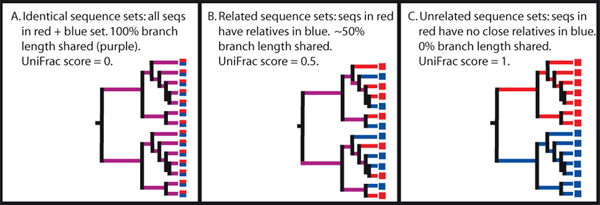
\includegraphics[width=80ex]{unifrac_test.jpg}
\end{figure}

For example, in the depiction, red branch lengths represent parts of the tree that extend from OTUs that are only present in one sample, blue branch lengths represent parts of the tree that extend from OTUs that are only present in the other sample, and purple branch lengths represent parts of the tree that extend from OTUs present in both samples. In the first image, \\
Here we present a proof that the UniFrac measurement is conformant with the triangle inequality, showing that it is a proper distance metric.

\section*{Proof}

We will examine perform the proof using three samples, $1$, $2$, and $3$, denoting the distances between them as $d_12$, $d_23$, and $d_13$. The triangle inequality is satisfied if we can show that $d_12 + d_23 \ge d_13$.\\
We can visualize the UniFrac method by putting all the branch lengths of the phylogenetic tree into a Venn Diagram.

\begin{figure}[h!]
  \centering
  \caption{Venn diagram of which samples the branch lengths in the phylogenetic tree belong to. The blue circle represents sample 1, the orange circle represents sample 2, and the green circle represents sample 3.}
    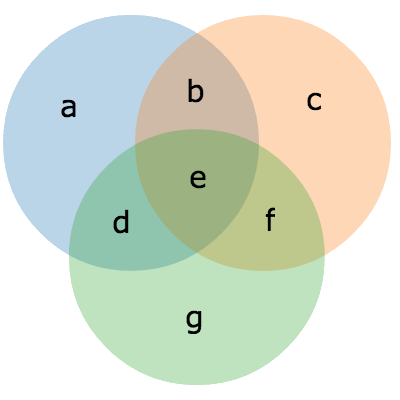
\includegraphics[width=80ex]{venn_diagram.png}
\end{figure}

Each circle of the Venn Diagram represents one sample. The region denoted by $a$ represents all the branch lengths of the tree that stem from OTUs present in sample $1$ but not any of the other samples. The region denoted by $c$ represents all the branch lengths of the tree that stem from OTUs present in sample $2$ but not any of the other samples. The region denoted by $g$ represents all the branch lengths of the tree that stem from OTUs present in sample $3$ but not any of the other samples. The regions $b$ and $e$ represent the branch lengths shared by samples $1$ and $2$, the regions $e$ and $f$ represent the branch lengths shared by samples $2$ and $3$, the regions $d$ and $e$ represent the branch lengths shared by samples $1$ and $3$, and the region $e$ represents the branch lengths shared by all three samples.\\[3ex]
The UniFrac distances between the samples are as follows:\\[1ex]
$d_{12} = \dfrac{sample\_1\_ and\_2\_unshared\_branch lengths}{sample\_1\_and\_2\_total\_branch\_lengths}$\\[1ex]
$d_{23} = \dfrac{sample\_2\_ and\_3\_unshared\_branch lengths}{sample\_2\_and\_3\_total\_branch\_lengths}$\\[1ex]
$d_{13} = \dfrac{sample\_1\_ and\_3\_unshared\_branch lengths}{sample\_1\_and\_3\_total\_branch\_lengths}$\\[3ex]
In terms of the regions of the Venn Diagram, this can be rewritten as:\\[1ex]
$d_{12} = \dfrac{a+c+d+f}{a+b+c+d+e+f)}$\\[1ex]
$d_{23} = \dfrac{b+c+d+g}{b+c+d+e+f+g}$\\[1ex]
$d_{13} = \dfrac{a+b+f+g}{a+b+d+e+f+g}$\\[3ex]
The Triangle Inequality can be formulated as follows:
$d_{12} + d_{23} \ge d_{13}$\\[3ex]
Substituting in the regions of the Venn Diagram:\\[1ex]
$\dfrac{a+c+d+f}{a+b+c+d+e+f)} + \dfrac{b+c+d+g}{b+c+d+e+f+g} \ge \dfrac{a+b+f+g}{a+b+d+e+f+g}$\\[1ex]
$\dfrac{a+c+d+f}{a+b+c+d+e+f)} + \dfrac{b+c+d+g}{b+c+d+e+f+g} - \dfrac{a+b+f+g}{a+b+d+e+f+g} \ge 0$\\[3ex]
Multiplying each term by $(a+b+c+d+e+f)(b+c+d+e+f+g)(a+b+d+e+f+g)$ to cancel out the denominators:
$(a^2b + a^2c + a^2d + a^2e + a^2f + a^2g + ab^2 + 2abc + 3abd + 2abe + 3abf + 2abg + ac^2 + 3acd + 2ace + 3acf + 2acg + 2ad^2 + 3ade + 4adf + 3adg + ae^2 + 3aef + 2aeg + 2af^2 + 3afg + ag^2 + b^2c + b^2d + b^2f + bc^2 + 3bcd + 2bce + 3bcf + 2bcg + 2bd^2 + 2bde + 4bdf + 2bdg + 2bef + 2bf^2 + 2bfg + c^2d + c^2e + c^2f + c^2g + 2cd^2 + 3cde + 4cdf + 3cdg + ce^2 + 3cef + 2ceg + 2cf^2 + 3cfg + cg^2 + d^3 + 2d^2e + 3d^2f + 2d^2g + de^2 + 4def + 2deg + 3df^2 + 4dfg + dg^2 + e^2f + 2ef^2 + 2efg + f^3 + 2f^2g + fg^2) +$\\[1ex]
$(a^2b + a^2c + a^2d + a^2g + 2ab^2 + 3abc + 4abd + 2abe + 2abf + 3abg + ac^2 + 3acd + 2ace + 2acf + 2acg + 2ad^2 + 2ade + 2adf + 3adg + 2aeg + 2afg + ag^2 + b^3 + 2b^2c + 3b^2d + 2b^2e + 2b^2f + 2b^2g + bc^2 + 4bcd + 3bce + 3bcf + 3bcg + 3bd^2 + 4bde + 4bdf + 4bdg + be^2 + 2bef + 3beg + bf^2 + 3bfg + bg^2 + c^2d + c^2e + c^2f + c^2g + 2cd^2 + 3cde + 3cdf + 3cdg + ce^2 + 2cef + 2ceg + cf^2 + 2cfg + cg^2 + d^3 + 2d^2e + 2d^2f + 2d^2g + de^2 + 2def + 3deg + df^2 + 3dfg + dg^2 + e^2g + 2efg + eg^2 + f^2g + fg^2) -$\\[1ex]
$(a^2b - a^2c - a^2d - a^2e - a^2f - a^2g - 2ab^2 - 3abc - 3abd - 3abe - 4abf - 3abg - ac^2 - 2acd - 2ace - 3acf - 2acg - ad^2 - 2ade - 3adf - 2adg - ae^2 - 3aef - 2aeg - 2af^2 - 3afg - ag^2 - b^3 - 2b^2c - 2b^2d - 2b^2e - 3b^2f - 2b^2g - bc^2 - 2bcd - 2bce - 4bcf - 3bcg - bd^2 - 2bde - 4bdf - 3bdg - be^2 - 4bef - 3beg - 3bf^2 - 4bfg - bg^2 - c^2f - c^2g - 2cdf - 2cdg - 2cef - 2ceg - 2cf^2 - 3cfg - cg^2 - d^2f - d^2g - 2def - 2deg - 2df^2 - 3dfg - dg^2 - e^2f - e^2g - 2ef^2 - 3efg - eg^2 - f^3 - 2f^2g - fg^2) \ge 0$\\[3ex]
This simplifies to:
$a^2b + a^2c + a^2d + a^2g + ab^2 + 2abc+ 4abd + abe + abf + 2abg + ac^2 + 4acd + 2ace + 2acf + 2acg + 3ad^2 + 3ade + 3adf + 4adg + 2aeg + 2afg + ag^2 + + b^2c + 2b^2d + bc^2 + 5bcd + 3bce + 2bcf + 2bcg + 4bd^2 + 4bde + 4bdf + 3bdg + bfg + 2c^2d + 2c^2e + c^2f + c^2g + 4cd^2 + 6cde + 5cdf + 4cdg + 2ce^2 + 3cef + 2ceg + cf^2 + 2cfg + cg^2 + 2d^3 + 4d^2e + 4d^2f + 3d^2g + 2de^2 + 4def + 3deg + 2df^2 + 4dfg + dg^2 + + efg + 2f^2g \ge 0$\\[3ex]
All the terms are positive, and all the regions contain positive branch lengths, therefore the inequality is true.

% Do NOT remove this, even if you are not including acknowledgments.
\section*{Acknowledgments}
Thanks to Mingchun Liu for helping me with the proof.

\nolinenumbers

%\section*{References}
% Either type in your references using
% \begin{thebibliography}{}
% \bibitem{}
% Text
% \end{thebibliography}
%
% OR
%
% Compile your BiBTeX database using our plos2009.bst
% style file and paste the contents of your .bbl file
% here.
% 
%\begin{thebibliography}{10}
%\bibitem{bib1}
%Lorem M, Ipsum VE (1990) Rank Correlation Methods. New York: Oxford University Press, 5th edition.
%
%\bibitem{bib2}
%Ipsum M, Ipsum JD (1990) Rank Correlation Methods. New York: Oxford University Press, 5th edition.
%
%\end{thebibliography}



\end{document}

